\scanpage{14}

\figure{
\begin{tikzpicture}\node[draw,circle,inner sep=3pt]{4};\end{tikzpicture}}
Supposons que $\unsure{U|\mathfrak g}=L_k(M)$, où $M$ est un $k$-
module, $U$ étant muni de la top. discrète.
Soit $\xi$ \uline{nilpotent} dans $U$, $g=\exp\xi$.
\[
\xi.a=0\quad\Longleftrightarrow\quad ga=a
\]
\[
\xi\text{ commute à }u\quad\Longleftrightarrow\quad g\text{ commute à }u
\]
\deleted{Supposons $\unsure{\xi}$}
\[
\begin{array}{ccc}
M'\text{ stable par }\xi&\Longleftrightarrow&M'\text{ stable par }g\\
(M'\subset M)&&
\end{array}
\]
\figure{\begin{tikzpicture}\draw[->](.3,0)..controls(-.2,0)and(0,.5)..(0,.8)--(0,1.5)--(.7,1.5);\end{tikzpicture}}

Supposons que $M$ soit muni d'une
application $k$-bilinéaire $(x,y)\longmapsto x.y$. Alors
\diagram{\[
\begin{array}{ccc}
\xi(x.y)=(\xi x)y+x(\xi y)&\Longleftrightarrow&g(x.y)=(gx)(g.y)\\
\uline{\text{dérivations}}&&\uline{\text{automorphismes}}\\
\text{nilpotentes}&&\text{unipotents}
\end{array}
\]}

\figure{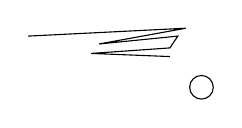
\begin{tikzpicture}\draw(0,.3)--(2,.4)--(.9,.2)--(1.9,.3)--(1.8,.15)--(.8,.08)--(1.8,.04);\draw(2.2,-.35)circle(.15);\end{tikzpicture}}

Soit $\Lambda$ une algèbre $k$-augmentée dont l'idéal
d'augmentation est \deleted{nilpotent}
\inserted{de puiss. n-ième nulle}, $k$ étant une
algèbre contenant $\mathbb Q$ \inserted{[donc $\Lambda$ contient $\mathbb Q$]},
Soit $M$ un $\Lambda$-module.
Alors les $u\in L_\Lambda(M)$ tels que $uM\subset I(\Lambda)M$
\inserted{i.e. $u$ induit $0$ dans $M\otimes_\Lambda k$}
sont nilpotents \deleted{\unsure{et les sont}}
\inserted{(de puiss. n-ième nulle)} les
$v\in L_\Lambda(M)$ tels que $v$ induise l'identité
dans $M\otimes_\Lambda k$ sont unipotents ; si \unsure{l'on}
\unsure{donne un nom à ces ensembles} $\unsure{\pi_k|\pi_\Lambda}$ resp\textsuperscript{t} $\gamma$,

\mspage{13}
